\documentclass[11pt]{article}
\usepackage[top=1.00in, bottom=1.0in, left=1.1in, right=1.1in]{geometry}
\usepackage{Sweave}
\renewcommand{\baselinestretch}{1.2}
\usepackage{graphicx}
\usepackage{natbib}
\usepackage{amsmath}
\usepackage{gensymb}
\usepackage{parskip}
\usepackage{xcolor}
\usepackage[disable]{todonotes}
\usepackage{lineno}
\usepackage{xr-hyper}
\newcommand{\R}[1]{\label{#1}\linelabel{#1}}
\usepackage{hyperref}
\usepackage[utf8]{inputenc}
\externaldocument{grephonsupp}

\def\labelitemi{--}
\parindent=0pt

\begin{document}

\renewcommand{\refname}{\CHead{}}

% See also: git/grants/crc2023/crc2023app/docs/crc_notes2023more.tex which has some reference notes

\begin{center}
{\sc Title:} {\Large Why longer seasons with climate change \\ may not always increase tree growth} \\
\vspace{5ex}
% Climate change highlights fundamental gaps in\\ plant growth $\times$ growing season length relationships  
% Do growing season length and growth relate? \\ And if not, why not? \\ And if we're not sure, why is that?
{\sc Authors:} E.M. Wolkovich$^1$, Ailene K. Ettinger$^2$, Alana Chin$^3$, Catherine J. Chamberlain$^4$,\\ Frederik Baumgarten$^1$, Kavya Pradhan$^{5,6}$, Rub{\'e}n D. Manzanedo$^{7-9}$ \&  Janneke Hille Ris Lambers$^7$
\end{center}

$^1$ Forest \& Conservation Sciences, Faculty of Forestry, University of British Columbia, 2424 Main Mall, Vancouver, BC V6T 1Z4, Canada\\
$^2$ The Nature Conservancy of Washington, 74 Wall Street, Seattle, WA  USA \\
$^3$ California State Polytechnic University, Humboldt. Department of Biological Sciences. Arcata, CA, USA \\
$^4$ The Nature Conservancy, 334 Blackwell St Ste 300, Durham, NC, USA \\ 
$^5$ Department of Biology, University of Washington, Seattle, WA, 98195 \\
$^6$ Moore Center for Science, Conservation International, Arlington, VA, 22202 \\ % kpradhan@conservation.org
$^7$ Institute for Integrative Biology, ETH Z{\"u}rich, 8092 Z{\"u}rich, Switzerland \\ %
$^8$ Institute of Plant Sciences, University of Bern, Bern, Switzerland \\
$^9$ Oeschger Center for Climate Change Research, University of Bern, Bern, Switzerland \\


% \emph{Data availability:}  No new data, but summarized data from literature review will be posted on KNB.


\newpage

% We are a review or perspective, see https://www.nature.com/nclimate/content ... either way we need to be 3-5K words
\begin{abstract} % 119 words and needs to be 120
% Here we highlight how widespread variation across studies may suggest the need for a path forward ... 
Most climate change forecasts assume that longer growing seasons increase carbon storage through increased tree growth, but recent findings have challenged this assumption. Here we highlight divergent findings across studies, spanning diverse methods and disciplinary perspectives. Current hypotheses for why longer growing seasons may not always increase tree growth include drought-related effects and internal constraints. These hypotheses, however, are generally tested in different ways by different fields on different species, and rarely consider how external drivers and internal constraints interact. We outline how bridging these divides while integrating evolutionary history and ecological theory could help build a unified model across species for when longer seasons will---or will not---lead to greater tree growth, with major forecasting implications.
% While studies have proposed  a suite of hypotheses for why longer growing seasons may not always increase tree growth, including drought-related constraints, internal limits, and methodological differences, comparing support for them is challenging given their diversity and that they were often confined to one sub-field: studies of tree ring growth tended to focus on external drivers, such as drought, while physiological studies of biomass or carbon allocation, tended to focus on internal limits, such as effects of photoperiod. 
% Two alternative endings:
% We argue that bridging disciplinary divides and integrating theory from community and phylogenetic ecology could help develop and test a mechanistic framework for when longer seasons will---or will not---lead to greater growth.
% We outline how bridging current disciplinary divides in hypotheses and methods while simultaneously integrating ecological theory could drive new advances in fundamental biology with major forecasting implications.  %...and help build a mechanistic framework for when longer seasons will---or will not---lead to greater growth, with implications of improve forecasts of forest responses and climate feedbacks in a warmer world.
\end{abstract}

\section*{Introduction} % 3 Jan 2025: 4087 plus Box

How plant growth shifts with warming has ramifications for the stability of ecosystems and the global climate system itself \citep{ipcc2021}. Because plants act as one of the greatest potential stores for carbon emissions how and how much their growth changes with climate change is one of the top predictors of future climate change \citep{ipcc2021,friedlingstein2022global}. The idea that longer growing seasons lead to increased plant growth is an intuitive tenet across multiple fields of biology, including physiology, dendrochronology and ecosystem ecology \citep{nobel1983biophysical,frank2022dendrochronology}. It is also a foundational assumption of many global carbon cycle models \citep[e.g.][]{ito2020global,friedlingstein2022global}. These models project that continued anthropogenic warming will be partly offset by increased carbon sequestration as warming lengthens growing seasons in many forests \citep{friedlingstein2022global}, an assumption supported by ecosystem-scale studies \citep{chen1999effects,keenan2014net,finzi2020}. 

Yet recent work has questioned this longstanding assumption \citep[e.g.][]{dow2022warm,green2022limits,silvestro2023longer}, challenging decades of research reporting increased growth with longer seasons, from observations along elevational and latitudinal gradients \citep[][]{myneni1997increased,berdanier2011growing,king2013tree,cuapio2022there}, classic experiments in lab settings \citep{went1957experimental}, to trends in ecosystem fluxes with warming \citep{chen1999effects,keenan2014net,finzi2020}. Proposed mechanisms for the apparent disconnect are diverse (Fig. \ref{fig:hypotheses}), including the complex nature of climate change \citep[e.g. drought or heat stress,][]{dow2022warm} and internal constraints on plant growth \citep{zohner2023effect}, which alone or interactively may limit plant responses \R{forbigKref1}\citep{korner2015paradigm}. % as well as inconsistent use of growth and growing season metrics and definitions \citep{green2022limits,korner2023four}.
% Studies that Green \& Keenan say no relationship:
	% Fatichi et al. 2014 (opinion)
	% Fatichi et al. 2019 (review)
	% JIang et al 2020 (FACE or sinilar) 

% Our approach spans multiple fields to unify foundational studies with recent research related to anthropogenic warming. Leveraging a systematic literature review, we examine in which methods, species and approaches extended seasons appear to lead to increased growth, and the current proposed hypotheses. 
Here we examine how different fields have studied the relationship between growing season length and tree growth to identify the potential mechanisms that unite---and could disconnect---these processes. % Our approach spans multiple fields, from foundational to recent studies.  
We find substantial variation in growth $\times$ season length relationships across different definitions (see Box: Defining the quest for a comprehensive framework across external and internal drivers). We also find a pervasive disciplinary split between studies, which test different mechanisms on different species. \R{fornccS}Current work often lacks a clear mechanistic physiological model \citep{korner2015paradigm,fatichi2019modelling}, and implicitly ignores the role of shared evolutionary history and community ecology to plant growth \citep[e.g.][]{Grime:1977sw,Webb:2002or,avila2023evidence}, which could slow the search for a universal model. We argue that a robust answer for whether longer seasons lead to increased growth will require new efforts and shifts in perspectives. Towards that aim, we outline how cross-disciplinary efforts to build a more mechanistic model across species, would allow the field to rapidly develop a framework to predict when, where and how climate change may increase tree growth.\R{fornccE} % Changes for Tegan here...

\section*{Evidence that longer seasons impact plant growth} % 58 char
%  (spanning 36 papers and 59 unique tests or studies; see Supp or Fig/Table)
The idea that time limits growth is a fundamental principle across biology. Many biological processes---including photosynthesis and aspects of growth---are rate-limited, making time a crucial commodity \citep{nobel1983biophysical,cosgrove2005growth,hilty2021plant}. Thus, the hypothesis that longer growing seasons should increase growth is intuitive---and pervasive. 

Foundational evidence comes from spatial clines across elevation and latitude, with growth decreasing alongside growing season length at higher elevations and latitudes (Fig. \ref{fig:gxelev}). Experimentally, this assumption is supported by small-scale field warming studies that find that phenologically advancing species also grow more with warming \citep[][]{Cleland:2012}, while observationally, ecosystem-scale studies have reported a similar relationship between season length and carbon fluxes across decades with global warming \citep{keenan2014net} or in years with warm, early springs \citep{chen1999effects}. However, some recent high-profile studies find no support for this relationship \citep{dow2022warm}. These studies, which often focus on inter-annual correlations with metrics of standardized individual tree growth \citep{dow2022warm,silvestro2023longer}, have generated debate about whether future carbon storage forecasts are overestimated and which metrics of growth \citep{green2022limits}, or growing season length \citep{korner2023four}, are relevant (see Box).

% ChangeBACK(postNCC)
% Despite this recent debate, we found that longer seasons lead to increased growth in a slight majority of papers spanning  25 years.
To better understand this recent debate we examined research spanning 25 years for current advances and potential gaps. Though the number of papers directly addressing this topic is small, a slight majority found that longer seasons lead to increased growth (21 of 36 total papers), with no clear pattern by method or year (Fig. \ref{fig:heatmaps} and see `Literature review methods' in Supplement). For example, carbon assimilation studies were evenly split in finding evidence for or against the relationship  (or simply not testing it, Fig. \ref{fig:heatmaps}). Diverging results occurred across and within methods, suggesting the drivers of this variation are likely due to biological mechanisms, not solely due to varying definitions of growth or growing season length \citep[as some have recently suggested, e.g.][and see Box]{green2022limits,korner2023four}. 

Most studies tested the hypothesis that longer seasons with climate change increase growth via either increased time to grow (10 of 36 papers) or because longer seasons are usually warmer (8 papers), although many also considered hypotheses that could disconnect growth from season length. Studies from dendrochronology (the study of tree rings and their dating) and physiology have readily offered explanations for findings that increased growth may not be a universal outcome of longer seasons (Fig. \ref{fig:hypotheses}). External climatic drivers that offset the positive growth effects of longer seasons were often reported in tree ring studies \citep{kolavr2016response,de2022temperature,camarero2022decoupled}. In particular, the hypothesis that higher temperatures paired with lower precipitation produce negative correlations of season length with growth appeared in 58\% of tree ring studies we reviewed (and was only mentioned once outside of these studies, see also Fig. \ref{fig:hypotheses}). In contrast, 43\% of lab experimental and wood phenology (xylogenesis) studies suggested fundamental internal constraints that prevent trees from responding to longer seasons \citep[Fig. \ref{fig:heatmapssupp},][]{cuny2012life,michelot2012comparing,zohner2023effect}. Yet we found that these hypotheses have been tested in radically different ways on different species, rarely together, and ignore relevant research from other disciplines. % As we outline below, a single mechanism is unlikely to explain all results, requiring a more unified framework---and tests of it---for progress. 
 
\section*{Controllers on growth $\times$ season length relationships} % 51 char

% A suite of mechanisms could prevent a universally positive growth $\times$ season length relationship. 
Major mechanisms that could limit or disrupt the positive effects of longer growing seasons generally fall into two categories: (1) external factors, such as drought, which should impact ecosystem-level trends at regional scales, and (2) internal physiological constraints, which some research suggests are either universal across plants \citep[e.g.][]{zohner2023effect}, or species- and population-specific \citep[e.g.][]{soolanayakanahally2013timing}. While we address each in turn, these drivers can clearly operate together \citep[][]{korner2015paradigm}\R{forbigKinteract1}, though research rarely teases them apart. Further, the importance of internal versus external drivers likely varies by species, highlighting the need to integrate perspectives from  phylogenetic and community ecology (we discuss these gaps further in `Building a new framework for growth $\times$ season length' below). 

\subsection*{External drivers}

% \paragraph{Temperature \& moisture} % Abiotic
Temperature limits many biological processes \citep{korner2015paradigm}\R{forbigKref0}. Temperatures that are too cool (below 5\degree C for temperate trees) and too warm \citep[an area of active research, but likely between 35-45\degree C;][]{martinez2008hot,cabon2022cross} slow down biological processes and eventually can lead to tissue death \R{morebox}\citep[see Fig. \ref{fig:moraconcept}a, Box,][]{larcher1980,kramer2012book}. Between these upper and lower limits, biological processes underpinning growth generally accelerate such that warming can have a direct effect by accelerating biological time, up until the maximum rate for that particular process. Assuming a common growth response curve to temperature, possible increased growth should be predictable based on the current seasonal temperatures and the amount of warming (Fig. \ref{fig:moraconcept}b). 

How much or whether growth increases at all depends on the non-linear effect of temperature on biological processes (Fig. \ref{fig:moraconcept}a). At very cool temperatures---such as in early spring---a small increase in temperature may have limited effect \citep[or even increase frost risk through early budburst, Fig. \ref{fig:hypotheses}e,][]{cat2021pep}, while an increase at warmer temperatures---such as those more common in the summer (e.g. 16 to 18\degree C)---could have a larger physiological impact. However, warming that pushes plants beyond their optima, where many biological rates crash, could have large negative impacts \citep{nobel1983biophysical,leuning2002temperature}. Thus, some studies hypothesize that longer seasons effectively only extend the very cool early-season periods and may have no discernible effect on growth (with varying definitions of growth, see Box), while other studies---based on tree rings---suggest that any increases in growth due to longer seasons can be offset by reduced growth due to high summer temperatures \citep[Fig. \ref{fig:hypotheses},][]{gantois2022new,dow2022warm}. In contrast, other researchers argue that warmer temperatures have not yet pushed trees above their optima \citep{schaber2002evaluation}, and instead have driven increases in growth through accelerated rates, rather than longer seasons \citep[e.g.][]{ren2019}, or through a combination of both.

Other external drivers could counteract positive effects of longer---or warmer---seasons on growth predicted from temperature responses alone. Moisture deficits from reduced precipitation or higher evaporative demand (commonly invoked in tree ring studies, Fig. \ref{fig:hypotheses}) can slow or stall growth. Support for this hypothesis comes from negative correlations between growth and precipitation \citep[or other metrics related to plant access to water in tree ring studies,][]{kolavr2016response,etzold2022number}, and is well supported by physiological observations  that water status can be a biophysical limit to growth \citep[i.e., cells cannot expand without sufficient turgor,][]{peters2021turgor,cosgrove2023structure}, though few physiological studies on season length considered this effect (Fig. \ref{fig:heatmaps}). \R{bigKextremeS}With increasing extremes in both temperature and moisture, understanding these factors \citep{schuldt2020first}---and how they interact---will become increasingly important \citep{charrier2021interaction}.\R{bigKextremeE} External biotic factors are also shifting with longer seasons---including herbivory, disease and competition\citep{mitton2012mountain,lange2006thresholds,cleland2024effects}---and can limit productivity \citep{sturrock2011climate,la2008forest,senf2017remote}, though they are missing from the current debate on the impacts of longer seasons on growth (we found no mention of them, Fig. \ref{fig:hypotheses}e). 

\subsection*{Internal constraints}
%  \paragraph{Universal limits \& triggers} 
When and how growth is initiated and ceases is under genetic and developmental control, and thus plants' internal programming could limit growth responses to longer seasons \citep{howe2003genotype}. Within species (intraspecifically) research has repeatedly shown that populations vary in their growth and responses to extended seasons, reflecting differences that likely evolved to limit tissue loss to rare early or late-season events \citep{mitton2012mountain,lange2006thresholds,cleland2024effects}. Populations often vary predictably in their end-of-season phenology, with more poleward populations tending to stop height growth (budset) earlier using locally adapted photoperiod cues \citep{soolanayakanahally2013timing,aitken2016}. This means longer seasons are generally driven by spring phenology, which appears far more flexible, and has advanced more rapidly than fall events \citep{aitken2016}. Some recent studies suggest novel roles for the summer solstice \citep{zohner2023effect} in setting a fixed universal developmental switch between when warming temperatures hasten or delay leaf senescence, and in determining when warmer temperatures trigger greater reproduction \citep{Journe2024}. % Within populations, individual trees may also vary in how early or late they initiate (spring) or end (fall) growth. This can be driven by a shifting investment to growth, survival and/or reproduction with growth. For example, saplings, for which growth and survival are paramount, tend to both grow more rapidly \citep{hilty2021plant} and have longer seasons relative to adult trees \citep{augspurger2003differences,rozendaal2010tropical,vitasse2014earlier}, which need to also invest in reproduction. % The response of adult trees may then vary depending on their investment in reproduction. 

Trade-offs between vegetative and reproductive investments may produce important growth response differences within individuals and  between species. Years of high reproductive output can reduce growth \citep{thomas2011bookchptr,hacket2016tree}. For species that mast---producing abundant cones or fruits in only some years---high reproduction could especially impact measures of wood growth. Higher summer temperatures may trigger masting in the following year \citep{hacket2016tree,hacket2016consistent}; if true, then reduced growth in years following warm summers may not indicate temperatures too high for growth, as recent studies have suggested \citep[e.g.][]{gantois2022new,dow2022warm}, but instead shifting investment to reproduction. Such contrasting interpretations of the same pattern highlight the lack of a comprehensive mechanistic model for how internal and external factors may operate---both independently and together---to affect the relationship between growth and season length \citep[see Box,][]{korner2015paradigm}\R{forbigKnomodel1}.

\subsection*{Species-level variation}
The effects of these external and internal drivers are likely to vary across species, with species identity strongly predicting variation in growth $\times$ season length relationships \citep[e.g.][]{cuny2012life,michelot2012comparing}. Though this reality was rarely acknowledged in studies we reviewed (Fig. \ref{fig:hypotheses}c), research in dendrochronology, physiology and in phenology often mentions important differences between certain species groups that should affect how longer seasons impact growth \citep{camarero2015or,fu2019nutrient,puchalka2024tree}. 

The distinct strategies of deciduous versus evergreen species, including in how and when they invest in leaf and shoot elongation versus cambial growth, can affect how they respond to longer seasons. While evergreen species generally leaf out later than deciduous species they can more immediately photosynthesize with earlier springs, though both types of species generally invest in buds (for new leaves, shoots and flowers) in the preceding year. This means neither can rapidly change their investment in leaf area in response to an earlier spring, but both can have multiple flushes of leaves \citep{day2011regulation,soolanayakanahally2013timing}. Wood growth in evergreen species is generally thought to come from current season photosynthates, while deciduous species may more often use stored carbon resources \citep{gordon1968seasonal,monson2018finding}. These differences would suggest season length by growth relationships
may be most apparent via lagged effects in deciduous species, but this is rarely studied  \citep[and not clearly supported to date, see][]{coulthard2020limits,klesse2023legacy}. % Further, evergreen species are thought to grow more slowly and thus differences due to season length may be harder to detect \citep{waring1979evergreen}.  

This division between evergreen and deciduous species hints at a larger suite of traits that predict growth by growing season length relationships among species. Species that budburst earlier and more readily produce additional leaves \citep[e.g. leaf flushes after budset, and other characteristics more common to `indeterminate' species,][]{kikuzawa1982leaf,Lechowicz:1984cr} may grow more with longer seasons (though potentially with a lag, see Box) versus those that budburst later and flush new primary growth only once. Similarly, species adapted to cold, dry or high latitude conditions may have different thresholds for when these external drivers limit or promote growth \citep[e.g. some \emph{Populus} and \emph{Quercus} species,][and see Fig.\ref{fig:moraconcept}]{soolanayakanahally2013timing,mckown2016impacts,delpierre2017tree,de2022temperature}. Such differences could easily obscure any overall relationship between growth and growing season length. Supporting this possibility, current studies finding divergent results (Fig. \ref{fig:sppfinds}) span a wide range of species (we found  57 species from 26 genera across 36 papers). 

\section*{Building a new framework for growth $\times$ season length} % 51 char

Understanding when, how and why longer seasons lead to increased tree growth would benefit from a framework that integrates across external and internal drivers to predict plant growth across species. \R{notallmech}While our brief review of this literature could not cover all possible mechanisms, it highlights disciplinary divergences and major gaps in our mechanistic model \citep[see Box, and ][]{korner2015paradigm,rossi2008critical,rademacher2022insights}\R{forbigKref1}\R{morebox1} that likely underlie the current debate in whether longer seasons lead to increased tree growth. We argue that a more mechanistic understanding of how these drivers integrate to explain current findings is possible, but will require new approaches that help address major open questions. 
% We argue that a more mechanistic understanding of how these drivers integrate over species diverse growth strategies and the imprints of evolutionary history to explain current findings is possible, but will require new approaches to help address major open questions. 


\subsection*{Integrate phylogeny and traits to guide research}  % xx char (Tegan suggested: integrate phylogeny and traits to identify gaps for research, but it's not a question) 
% How do species responses map onto traits and phylogeny? % 55 char
%From Ailene 5/20/2025: I think I like this subheading, but here are some alternative subheading ideas:
%Can we leverage the diversity of species responses to inform a universal model for how growing season length influences growth?
%Predicting when and where longer growing seasons will lead to increased growth would benefit from a framework that leverages species variation to understand when external and internal drivers limit growth. 
% Useful models of tree growth for climate change forecasting must include a diversity of species, while overcoming the challenges of uneven sampling across species and their contrasting responses. 
The diversity of responses across species is a major challenge to building a common framework to predict how growth shifts with growing season length. Different species---especially those with different growth strategies \citep{Grime:1977sw}---are unlikely to have the same response to longer seasons, thus results of studies on one species may not easily translate to another. Yet explicitly incorporating this diversity could offer a path to connecting apparently divergent results. 

New approaches that integrate how species traits and evolutionary history shape responses to climate change  \citep{cornwell2017phylogenetic,harmonebook} could organize responses to provide novel insights and guide new studies. In particular, advances in phylogenetic comparative methods \citep{Webb:2002or} have moved research away from treating species identity as a simple grouping factor where each species is unique (e.g. \emph{Fagus sylvatica} is different from \emph{Quercus robur} and \emph{Pinus sylvestris}) or fits into a limited set of groups (e.g. deciduous versus evergreen) and towards species as suites of correlated observations, separated by their evolutionary distance (e.g. \emph{Fagus sylviatica} is much more closely related to \emph{Quercus robur} compared to \emph{Pinus sylvestris}). This evolutionary distance may explain diverging responses, but can also help identify underlying growth strategies that drive species- and clade-level variation \citep[][]{pearse2019interaction,morales2024phylogenetic}. Such models can layer in species-level information, such as traits correlated with differences in growth strategies, while phylogeny can capture additional species differences, which likely capture unmeasured `latent' traits . 

%Ailene added 5/20/2025: you could cut the below paragraph, i think, if you need to cut something in this section.
% Lizzie (21 May): Yes!
% In step with these advances, trait ecology has documented leaf and wood economic spectra that suggest major traits that underlie different strategies and could be included in these models \citep[with related databases of these traits often available,][]{Chave2009,diaz2016}. These `economics' define a common trade-off along an acquisitive to conservative axis, where some species grow rapidly and more flexibly to take advantage of resources, but are less defended against herbivores and compete poorly at low resource levels, whereas other species compete well at low resource levels, but at the expense of growing slower  \citep[][]{Grime:1977sw,Chave2009,diaz2016}. While these traits likely miss critical components for understanding how growing season length shapes growth, such as when different species invest in shoot and leaf versus wood growth, they provide a baseline from which to build, and a powerful approach to combine data usefully across species. This approach has already been used to identify that early-leafout species often show faster-growing more acquisitive strategies compared to later-leafout species \citep[reviewed in][]{cleland2024effects}---differences that may also impact how they respond to longer seasons. 
% While evolutionary distance often predict a suite of important species traits---and possibly also unmeasured latent traits (CITES)---ecophylogenetics incorporates both for a more useful and predictive framework.

In addition to naturally organizing species differences, a trait-based phylogenetic comparative approach can help build a more testable and predictable framework. % that can more readily forecast species responses ... 
Because this approach can flexibly fit evolutionary history and traits together, it allows clades or species groupings that respond similarly to emerge from the data and models \citep{davies2019phylogenetically}, versus being a priori grouped or defined. Similarly traits that co-vary with different responses can be more quickly identified \citep[e.g.][see Fig. \ref{fig:phylomodel}]{willis2008phylogenetic,davies2019phylogenetically}. Both of these benefits could highlight which species or traits to focus additional studies on to gain the most insights, while similarly suggesting areas that should be less studied \citep[e.g. traits that may be too confounded with evolutionary history,][]{cornwell2014functional,westoby2023phylogenetically} or outlier species that may not represent most species \citep{morales2024phylogenetic}. This approach may thus redefine debates over which metrics of growth or growing season length are relevant into debates over which metrics are most relevant for which clades and/or traits (see Box). % It could also help guide research to address what we argue are three major open questions.

% Predicting when and where longer growing seasons will lead to increased growth---or not---is possible with focused efforts to partition variation to different drivers in a framework that leverages species variation. 
% Because species diverge strongly in their growth and investment strategies any search for a common model will need to leverage this variation, as opposed to ignore it ... 

\subsection*{Testing for constraints across species and populations} % 60 char (removed 'internal')

% Predicting changes in growth in response to longer seasons requires understanding how much variation is possible inter-annually, within individuals. 
New evidence suggests inter-annual variation in growth may be limited because of internal constraints that prevent plants from fully using longer seasons \citep{zohner2023effect}. If true, this would have major ramifications for how much we expect growth to shift with warming. All plants are limited by internal constraints and how quickly they can build new tissues \citep{marchand2021timing,luo2024internal}, but selection towards different growth strategies (e.g. acquisitive versus conservative) should drive variation in these constraints across species. Selection should also drive local adaptation in these constraints at the population-level \citep{mckown2016impacts,soolanayakanahally2013timing}, by favoring individuals that match to local environmental optima \citep{Colautti:2010,mckown2014np}. This appears to be the case for budset---which indicates the end of height growth, though we currently have data on only a few species \citep{aitken2016,zeng2024weak}. 

New studies could rapidly test for constraints across species and populations to work towards a predictive framework using phylogeny and traits to predict these constraints. This approach has already yielded useful insights in spring phenology, highlighting which environmental factors consistently drive budburst across species while also showing widely-cited results may not extend beyond one well-studied species \citep{morales2024phylogenetic}. Organizing current data for budset and other metrics of start and end of growth (see Box) could identify how variable responses are across populations and species. 

\R{moconstrainS}The best tests of constraints will likely leverage experiments. Large-scale common garden studies can test for constraints in adult trees, including constraints due to different strategies and from past climatic events \citep[e.g., by selecting species with different growth strategies and/or selecting populations within a species with varying past exposure to damaging early season frosts][]{charrier2015effects,tixier2020comparison}. Such approaches take time, but could be supplemented by manipulative experiments. While juvenile stages of trees are often more flexible than their adult forms, they usually provide predictable inference in differences across species and populations, and thus should be integrated far more into studies of how season length affects growth. Using saplings and controlled environments could quickly test how much growth can---or cannot---shift with longer seasons---providing a potentially standardized way to compare constraints across species and populations.\R{moconstrainE} 

% Further, many results often schmear across species and populations \citep[e.g. studies using NDVI,][]{zohner2023effect}, but new studies could rapidly test for 
% From JHRL but not added (yet) for space: Interestingly, our review of the literature suggests that surprisingly few manipulative experiments of this kind have explicitly sought to test hypotheses that allow us build a more generalizable understanding of how growing season length influences growth.    

\subsection*{Identifying the scale of variation across space and time} % 53 char (What is the scale of variation across space and time? ... Was: What is the scale of variation in season length x growth relationships across space and time? Tegan suggested: use tree ring across climate gradients to understand possible effect sizes')

The idea that growing season length influences plant growth is fundamental to plant biology, but we found it is rarely tested in ways relevant to the current debate (see `Growth $\times$ elevation relationships' in Supplement)---a major gap that limits progress. While multiple papers report a lack of relationship between growth and growing season length (Figs. \ref{fig:hypotheses}, \ref{fig:heatmaps}), we have no fundamental understanding of what the effect size of this relationship should be, and thus no way to know if we have sufficient power in current studies to detect it. % Additionally, understanding large-scale pattens often improves models of the underlying processes, by finding unexpected trends or highlighting covarying drivers that must be disentangled. % ; for example, it may force a more immediate efforts to tease out effects of growth rates versus longer seasons. 

Identifying the macro-scale pattern is a tractable way to help develop a framework for growth $\times$ growing season length relationships. Tree ring studies designed to leverage latitudinal and elevational gradients in climate could quickly provide the raw data \citep{manzanedo2024moving}. Research will then need to develop models that tease out the effects of warmer temperatures across the season---likely affecting important biological rates  (Fig. \ref{fig:moraconcept})---versus longer seasons. Disentangling these may require focused efforts to understand xylogenesis across species and climates, but doing so across major climatic gradients could make differences more obvious. Wood growth provides an obvious baseline from which to set expectations of how much growth can vary across space, and links to existing major datasets (Fig. \ref{fig:itrbdpep}).  Research will also then need to integrate beyond wood growth, including methods to better characterize changes across the leaf, shoot and wood architecture of different species \citep[e.g.][]{puletti2020lidar,sillett2024ground} and also extending to the complexity of roots \citep{mckown2016impacts,radville2016}. These data can provide a baseline to compare to the scale of shifts over time, which studies of growth $\times$ growing season length to date have focused on (Fig. \ref{fig:heatmaps}), since the same tree rings measured for understanding spatial variation will also capture inter-annual variation. %Ailene added: could cite this reference here: https://onlinelibrary.wiley.com/doi/abs/10.1111/gcb.15170

% To answer this: go out and observationally measure the same species across latitude or elevation and aim to measure the RATE and TIMING of primary and secondary growth (getting at total SUM across season). 

% Start with tree rings for this and then break it down by types of growth, GSL metrics etc. (Nail this pattern across space and species; and then fit in what we see/expect over time). 

\subsection*{Interactions between external drivers and internal constraints} % 58 char  (Was: How do external drivers and internal constraints act together?)

% Most research on how growth impacts growing season length with climate change has been focused on either external or internal drivers. Certain studies have documented potential constraints while others focused on teasing out how temperature, drought and other external forces impact growth. Inherently, however, external and internal factors are interconnected and thus any useful model must include both together.  We argue that understanding the pattern across space---and using it benchmark the possible magnitude of inter-annual responses---alongside documenting the scale of internal constraints across species and populations will be critical to help compare responses of external and internal drivers. As these new data come together with trait-mediated phylogenetic models, we expect real advances will require more experiments across scales and disciplines.  

The external and internal factors that affect how longer seasons impact growth are inherently interconnected \citep{nobel1983biophysical}. While research often acknowledges this, modeling these together will require new experiments and observational studies, ideally designed to integrate into trait-mediated phylogenetic models. Studies across space could provide inference by studying how growing seasons measured by vegetative versus wood phenology vary---and attributing variation through models that nest populations within species and include traits while also testing for how climate drives growth.  
% But it needs a lot more work to understand if (a) it is common across species, and populations (partition variance) and (b) holds up under different definitions of GSL (c) is backed up experimentally (Figure showing what we expect from experiments maybe?).

The complexity of climate change and plant growth in response to longer, warmer seasons makes experiments vital to building useful mechanistic models for understanding current trends and for forecasting. Observational data---used mainly to date to tackle this question (Figs. \ref{fig:heatmaps}, \ref{fig:heatmapssupp})---generally confounds multiple external drivers, including season length, temperature and precipitation regimes \citep{ren2019,ipcc2021,camarero2022decoupled}, making it impossible to tease out actual drivers behind observed trends. Experiments, in contrast, can provide more robust tests and help understand observational responses. Experiments that we outlined to test for internal constraints in saplings (above) can layer on shifts in external drivers to tease apart this complexity. Combining results from such experiments with observational data from larger-scale well designed networks \citep[see][]{schuldt2020first} could be transformative.\R{bigKextreme2} % Such studies could also begin to tease out effects of increased growth rates due to warmer temperatures versus longer seasons. 

Building a better mechanistic model of tree growth will also require teasing out changes in season length from warming that affects rates; a challenge best addressed by new experiments that decouple these two factors. Such experiments could start on juvenile trees to help inform the underlying model, select representative species to focus on, and  develop predictions for large-scale studies. Experiments could also inform a better model of lag effects across species, with small-scale studies sampling saplings multiple years after manipulations (versus the common practice of destructive sampling at the end of the treatment growing season) and large-scale studies following existing efforts to test for ecological `memory'  \citep[e.g. ][]{flinker2021promise,schweiger2022transgenerational,chinmemory}. These efforts should help bridge across the contrasting timescales of current physiological and dendrochronological studies of growing season length: we found most physiological studies of growth $\times$ growing season length relationships studied 1-2 years of dynamics, usually of juvenile trees, while tree ring studies focused on synthesizing across decades of adult tree growth.

Expanding studies across more species will support development of accurate models that can forecast at relevant scales and to help design large-scale experiments. While experimenting on adult trees is difficult, previous challenges in climate change research have led to large-scale experiments to understand other complex drivers \citep[e.g. SPRUCE, DroughtNet, Pfynwald,][]{norby2011ecological,hanson2017attaining,smith2016drought}. We expect similar experiments will be critical here. Preparing for these large experiments using trait-mediated phylogenetic models to understand responses across species, however, could yield advances well beyond past efforts. By informing which species or clades to study, new experiments could span enough phylogenetic and trait diversity to forecast species beyond the experiment and maximize the information gained \citep{cadotte2017phylogenies}. 

Starting now to leverage data across species to inform and design new large-scale studies and experiments will help build accurate models of future forest and related carbon dynamics, with implications for projections of carbon sequestration, carbon markets and climate stability. Emissions reduction and mitigation strategies today depend on growth and yield models built on assumptions that---if incorrect for certain species, regions or climate change scenarios---could endanger the success of current efforts \citep{ellis2024principles}. Thus, we argue that starting now to gather better data, build better models to improve our understanding of how climate change has and will impact tree growth is critical to durable and resilient policies to limit and adapt to future climate change.

% Anthropogenic climate change has often been described as an unfortunate and unplanned experiment. Like many experiments, it has highlighted important biology we do not know well. 
 
% 13 May 2024: Lizzie deletes conclusions. One sentence tagged onto end of last paragraph above, and the rest moved up (or deleted for future section). 
% My version: The task may seem large, but bridging across theory and data from dendrochronology, physiology, community and phylogenetic ecology could rapidly advance fundamental biology in ways that translate directly to improved models of future forest dynamics, with implications for and projections of carbon sequestration and carbon markets as well.  And that includes carbon sequestration---which, we really need now! 

% Ailene's version: Understanding when, how and why longer seasons lead to increased tree growth requires an interdisciplinary reckoning with how temperature, time and a suite of external and internal drivers affect plant growth. A mechanistic understanding of how these drivers integrate to affect growth will be critical for generating accurate global carbon forecasts biophysical feedbacks from future climate change, with implications for and projections of carbon sequestration and carbon markets as well. 

% Most fields studying growth $\times$ growing season length relationships consider a limited set of metrics and a small subset of possible drivers (see Figs. \ref{fig:heatmaps}, \ref{fig:heatmapssupp}). Beyond failing to test a suite of highly relevant mechanisms, the lack of interdisciplinary study means we lack coherent tests that compare multiple mechanisms. Taken together, the current landscape of research suggests we may be testing hypotheses for how plants shift with climate change that we never previously understood well in fundamental biology.
% Most fields studying this include a limited set of metrics and consider only a small subset of potential factors, with entire suites of hypotheses missing from the literature (see Fig. XX). 

% Beyond failing to test a suite of highly relevant mechanisms, the lack of interdisciplinary study means we lack coherent tests that compare multiple mechanisms. Dendrochronology considers almost exclusively external climatic drivers, while physiological tests of constraints do not usually predict for which species, when and where constraints will be most important. Taken together, the current landscape of research suggests we may be testing a hypothesis for shifts with climate change that we never previously understood well in fundamental biology. 

\emph{Acknowledgements:} B. Wuu for extracting growth $\times$ elevation data; R. Z{\"a}ch for logistical support; N. Pederson for discussion, J. Davies and three reviewers for comments that improved the manuscript. Support provided by the Rubel Foundation (JHRL), NSERC Discovery (EMW) and the Swiss State Secretariat for education, Research and Innovation (SERI) by a SERI-funded ERC Starting Grant #MB23.00011 (RM). \\

\emph{Author contributions:}  All authors conceived of the idea, prepared the literature review, edited the manuscript and contributed to designing some of the figures; in addition EMW wrote the manuscript, AKE, AC, CJC  and EMW synthesized the literature review, RD led developing Fig. \ref{fig:hypotheses}, CJC developed Fig \ref{fig:heatmaps}, EMW developed Fig. \ref{fig:phylomodel}, and AC, RD and EMW led developing the Box figure and Fig. \ref{fig:moraconcept}. 

\emph{Conflict of interest:} The authors declare no conflict of interest.  

\newpage
{\bf Box. Defining the quest for a comprehensive framework across external and internal drivers}
\begin{figure}[h!]
\includegraphics[width=0.95\textwidth]{..//figures/gslconcept/NEW_FI~1_ac_ver3.1.png}
\label{fig:defineGSLgrowth}
\end{figure}

\R{forbigKref2S}The idea that plants would not clearly benefit from the temporal opportunity to photosynthesize more has highlighted the lack of a comprehensive model of tree growth. This has ignited a series of debates on the fundamental biology of how trees grow, including over the importance of source (photosynthesis-limited) versus sink limitations \citep[plant growth-limited, but often via temperature, biophysical constraints, nutrients, and other arguably external factors,][]{korner2015paradigm,fatichi2019modelling,rademacher2022insights,cabon2022cross}\R{forbigKref2E} and which metrics of growth and growing season length are relevant. Yet the complexity of each term means that neither can have one simple definition. 

Here we show the simplified climate of one year (a), which determines rates and timing (b) of primary growth (root and shoot elongation and leaf production from meristems) and secondary growth (radial wood and bark growth from cambia), both of which often depend on conditions determining non-structural carbohydrate \citep[NSC, which are sugars and starch needed for growth and an important area of study, for more details see][]{hartmann2016understanding,martinez2016dynamics,tixier2020comparison,luo2024internal} production and reserves and storage from previous seasons. \R{forbigKNUTS1}Assuming sufficient available nutrients \citep{korner2015paradigm}, each of these types of growth could define the growing season length (GSL, c) but GSL can also be defined meteorologically (shown here as time, $t$, above some minimum $X$\degree C and below above some maximum $X$\degree C, with sufficient soil moisture) or by large-scale measures of plant productivity \citep{korner2023four}. Lagged effects (shown in gray in b) are lasting impacts of previous time periods either in the form of NSC stores or structural legacies influencing productivity. 

Of studies in our literature review, the largest proportion used metrics related to secondary growth, quantifying growth by measuring radial growth (e.g. through increment cores or dendrometers, $n=$28), but a number also looked at metrics related to primary growth, including C assimilation (e.g. net ecosystem productivity or gross primary productivity, $n=$20). For growing season length, the largest number of studies used vegetative (e.g. budburst to leaf senescence in our figure above, 26 studies) or wood phenology (11 studies) as their definition, while a smaller number used a meteorological definitions or fixed dates (7 studies). We found 14 studies that did not directly measure GSL \citep[e.g.][]{zhu2021different,dow2022warm,zohner2023effect}. 

\R{forbigKNUTSetcS}These different metrics limit any current effort to synthesize results across studies (see `The challenge of metrics: Measuring growth and growing season length' in the Supplement) but also highlight a limited mechanistic framework of tree growth at the physiological level \citep{korner2021tools,manzanedo2024moving}. \R{notallmech2}While we cannot integrate over all the proposed mechanisms that could help define these terms to improve our model of growth, research designed to test links between metrics and the physiological processes associated with external drivers and internal constraints would aid progress \citep{vieira2020tree}. For example, some meteorological definitions could relate directly to temperatures that limit cell growth, as multiple studies suggest growth stops at below $5$\degree C \citep{korner1998re,rossi2008critical}, but we need more studies of the upper limit and a better framework to test for variation across species. Layering on what levels of nitrogen, micronutrients and drought are also critical thresholds for growth \citep{korner2022forest,el2022accumulation,fu2019nutrient} should help predict variation across space and species, but a full framework would benefit from an improved understanding of how growth and stress operate at the cellular and molecular levels \citep{nilsson2008dissecting,ye2015molecular,rademacher2022insights}.\R{forbigKNUTSetcE}


\clearpage
\section{References}
\bibliography{..//bibtex/grephonbib}
\bibliographystyle{naturemag} % {/Users/Lizzie/Documents/git/bibtex/styles/naturesupp.bst} 


\clearpage
\section{Figures}
% 30 May 2024: Ruben updated figures to make them look better. I have kept the new paths and left the old paths below so we have them.

\begin{figure}[h!]
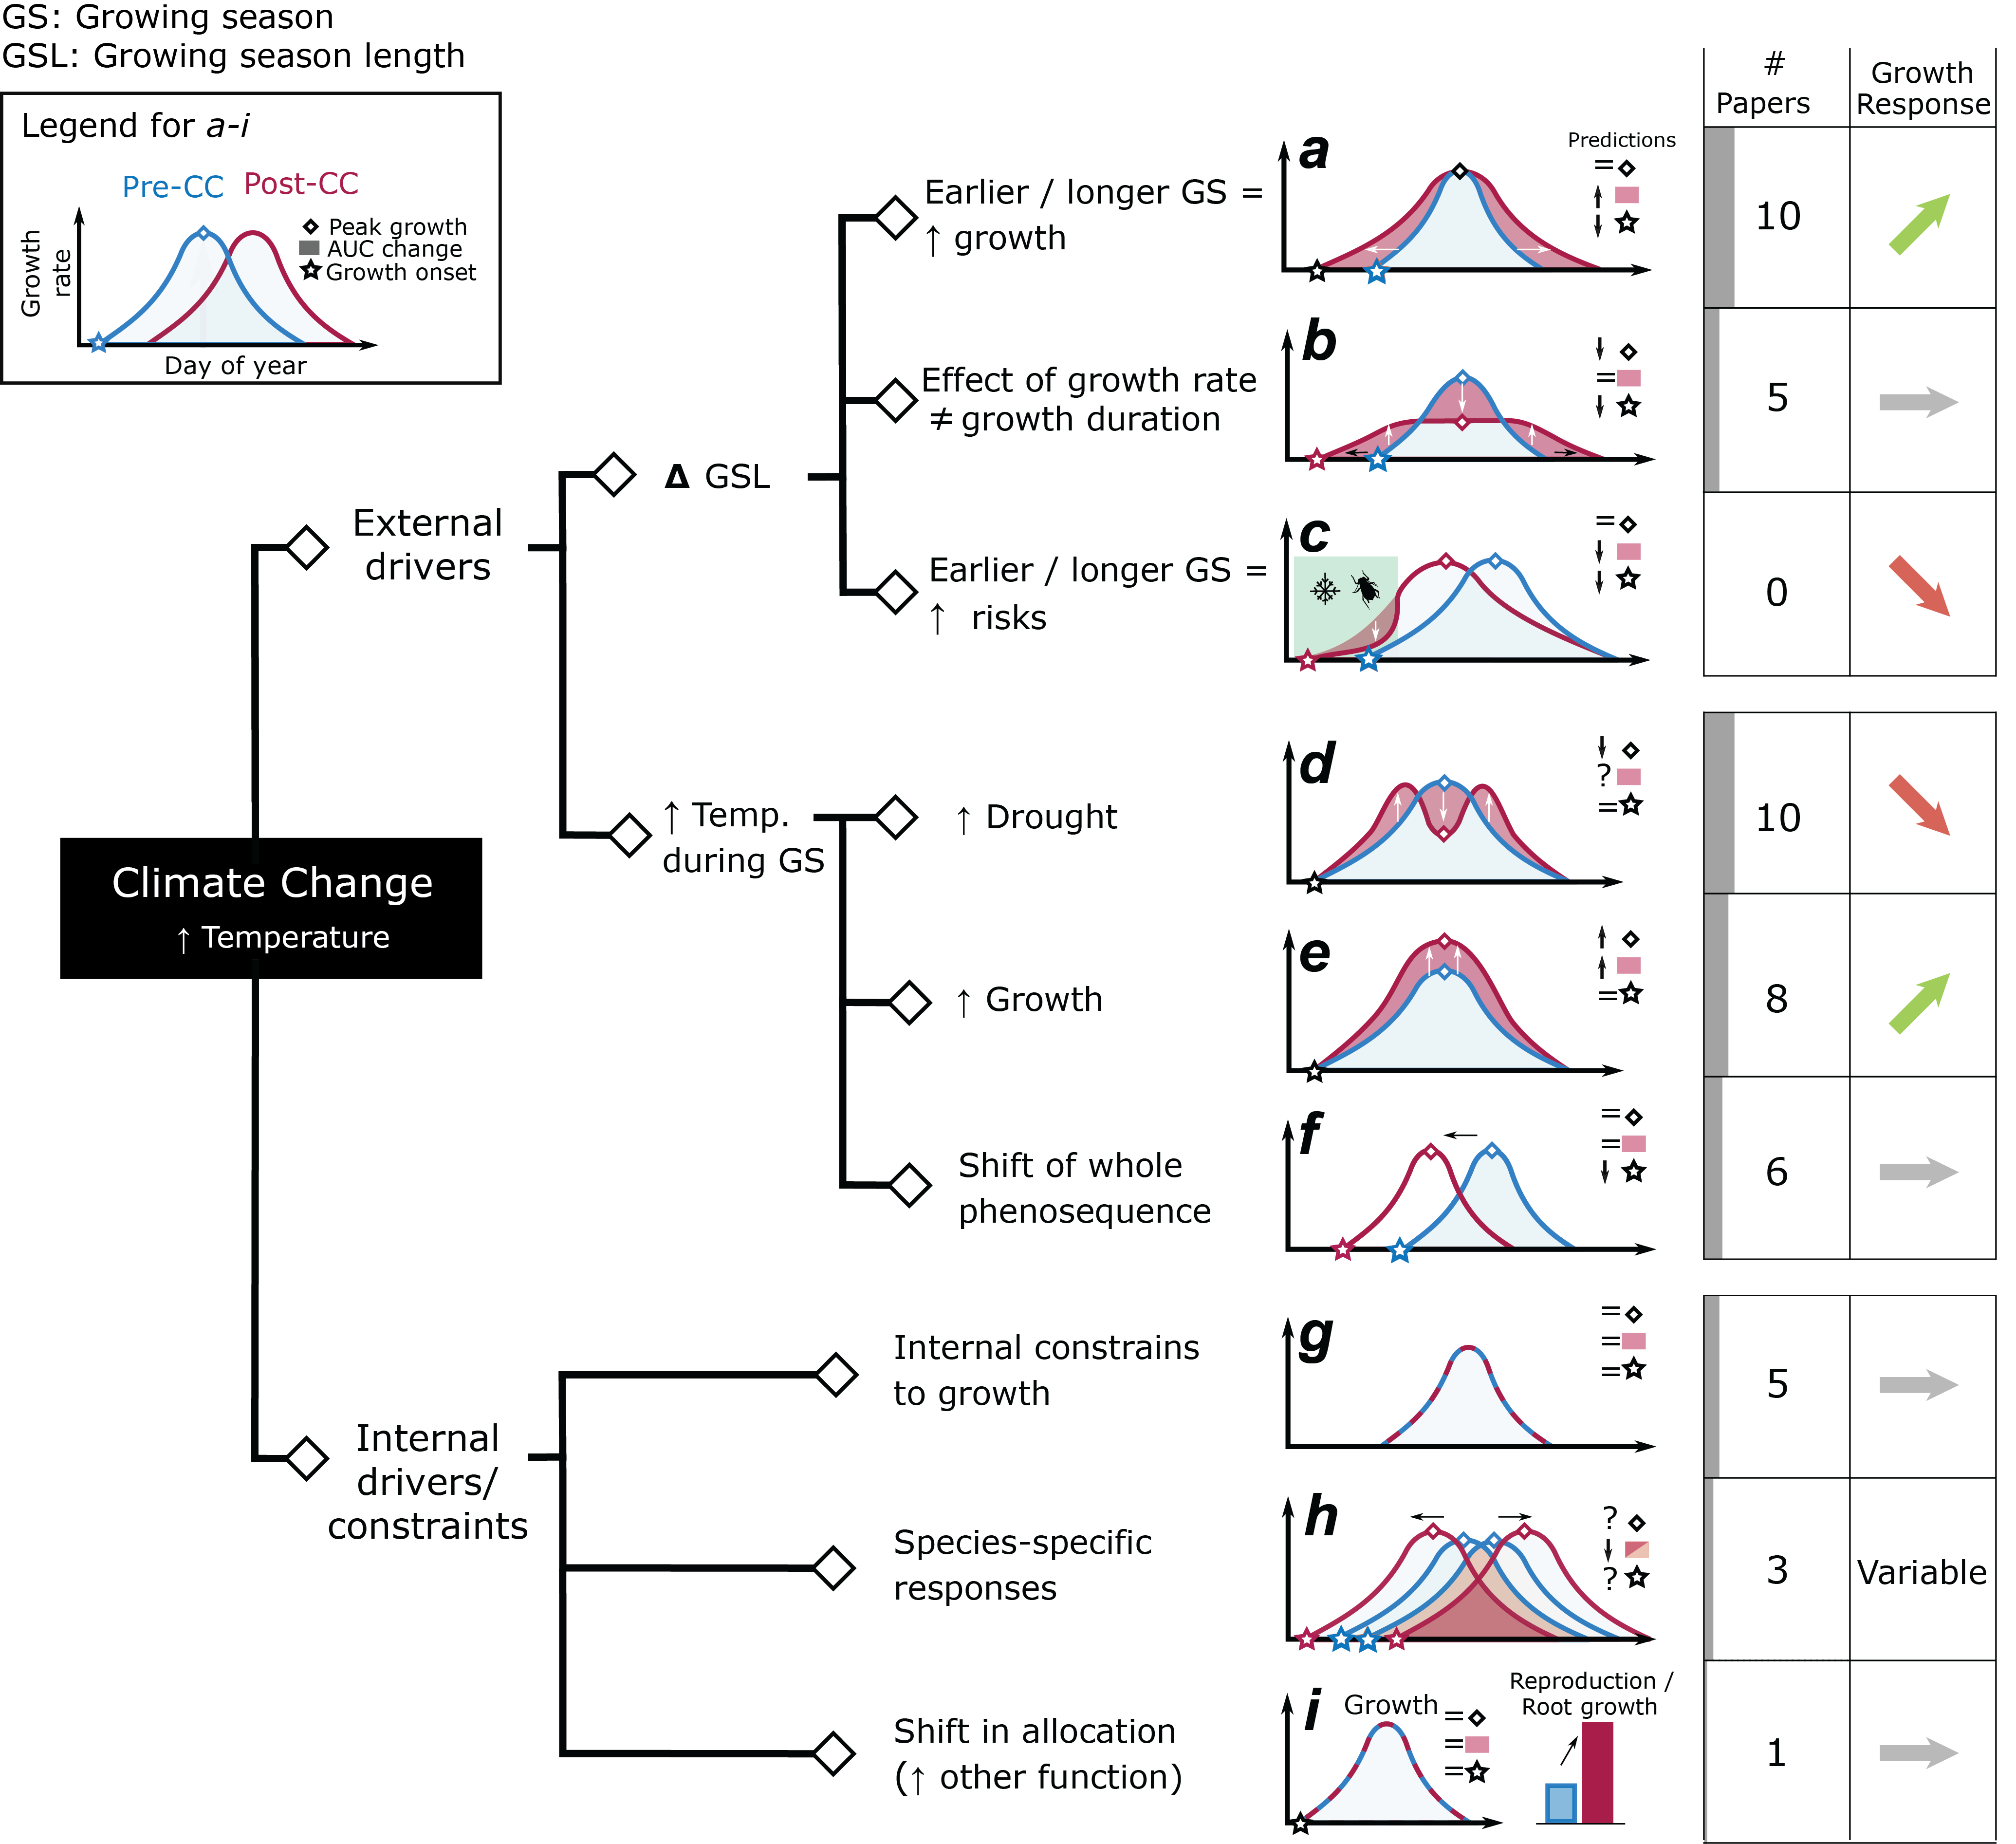
\includegraphics[width=0.9\textwidth]{..//figures/_figuresFromRuben/conceptualRev.png}
\caption{\emph{Altered growing season length (GSL) due to climate change can affect tree growth through diverse pathways.} We review hypotheses for these pathways showing the number of papers (from a review of papers studying growth $\times$ growing season length) that mentioned each hypothesis. For each graph, the peak (diamond), growth onset (start), and change in area under the curve (shading) is highlighted for the growth curves before (blue) and after (red) climate change. The right side columns highlight the number of papers studying each mechanism (left) and the expected growth response for each hypothesis (right). We group hypotheses as focused on mechanisms moderated by the environment (`external') versus those focused on internal physiological constraints, which span both source (photosynthesis-limited) and sink limitation, and could act together. For more details, see Supplement.} 
\label{fig:hypotheses}
\end{figure}

\clearpage
\begin{figure}[h!]
\label{fig:heatmaps}
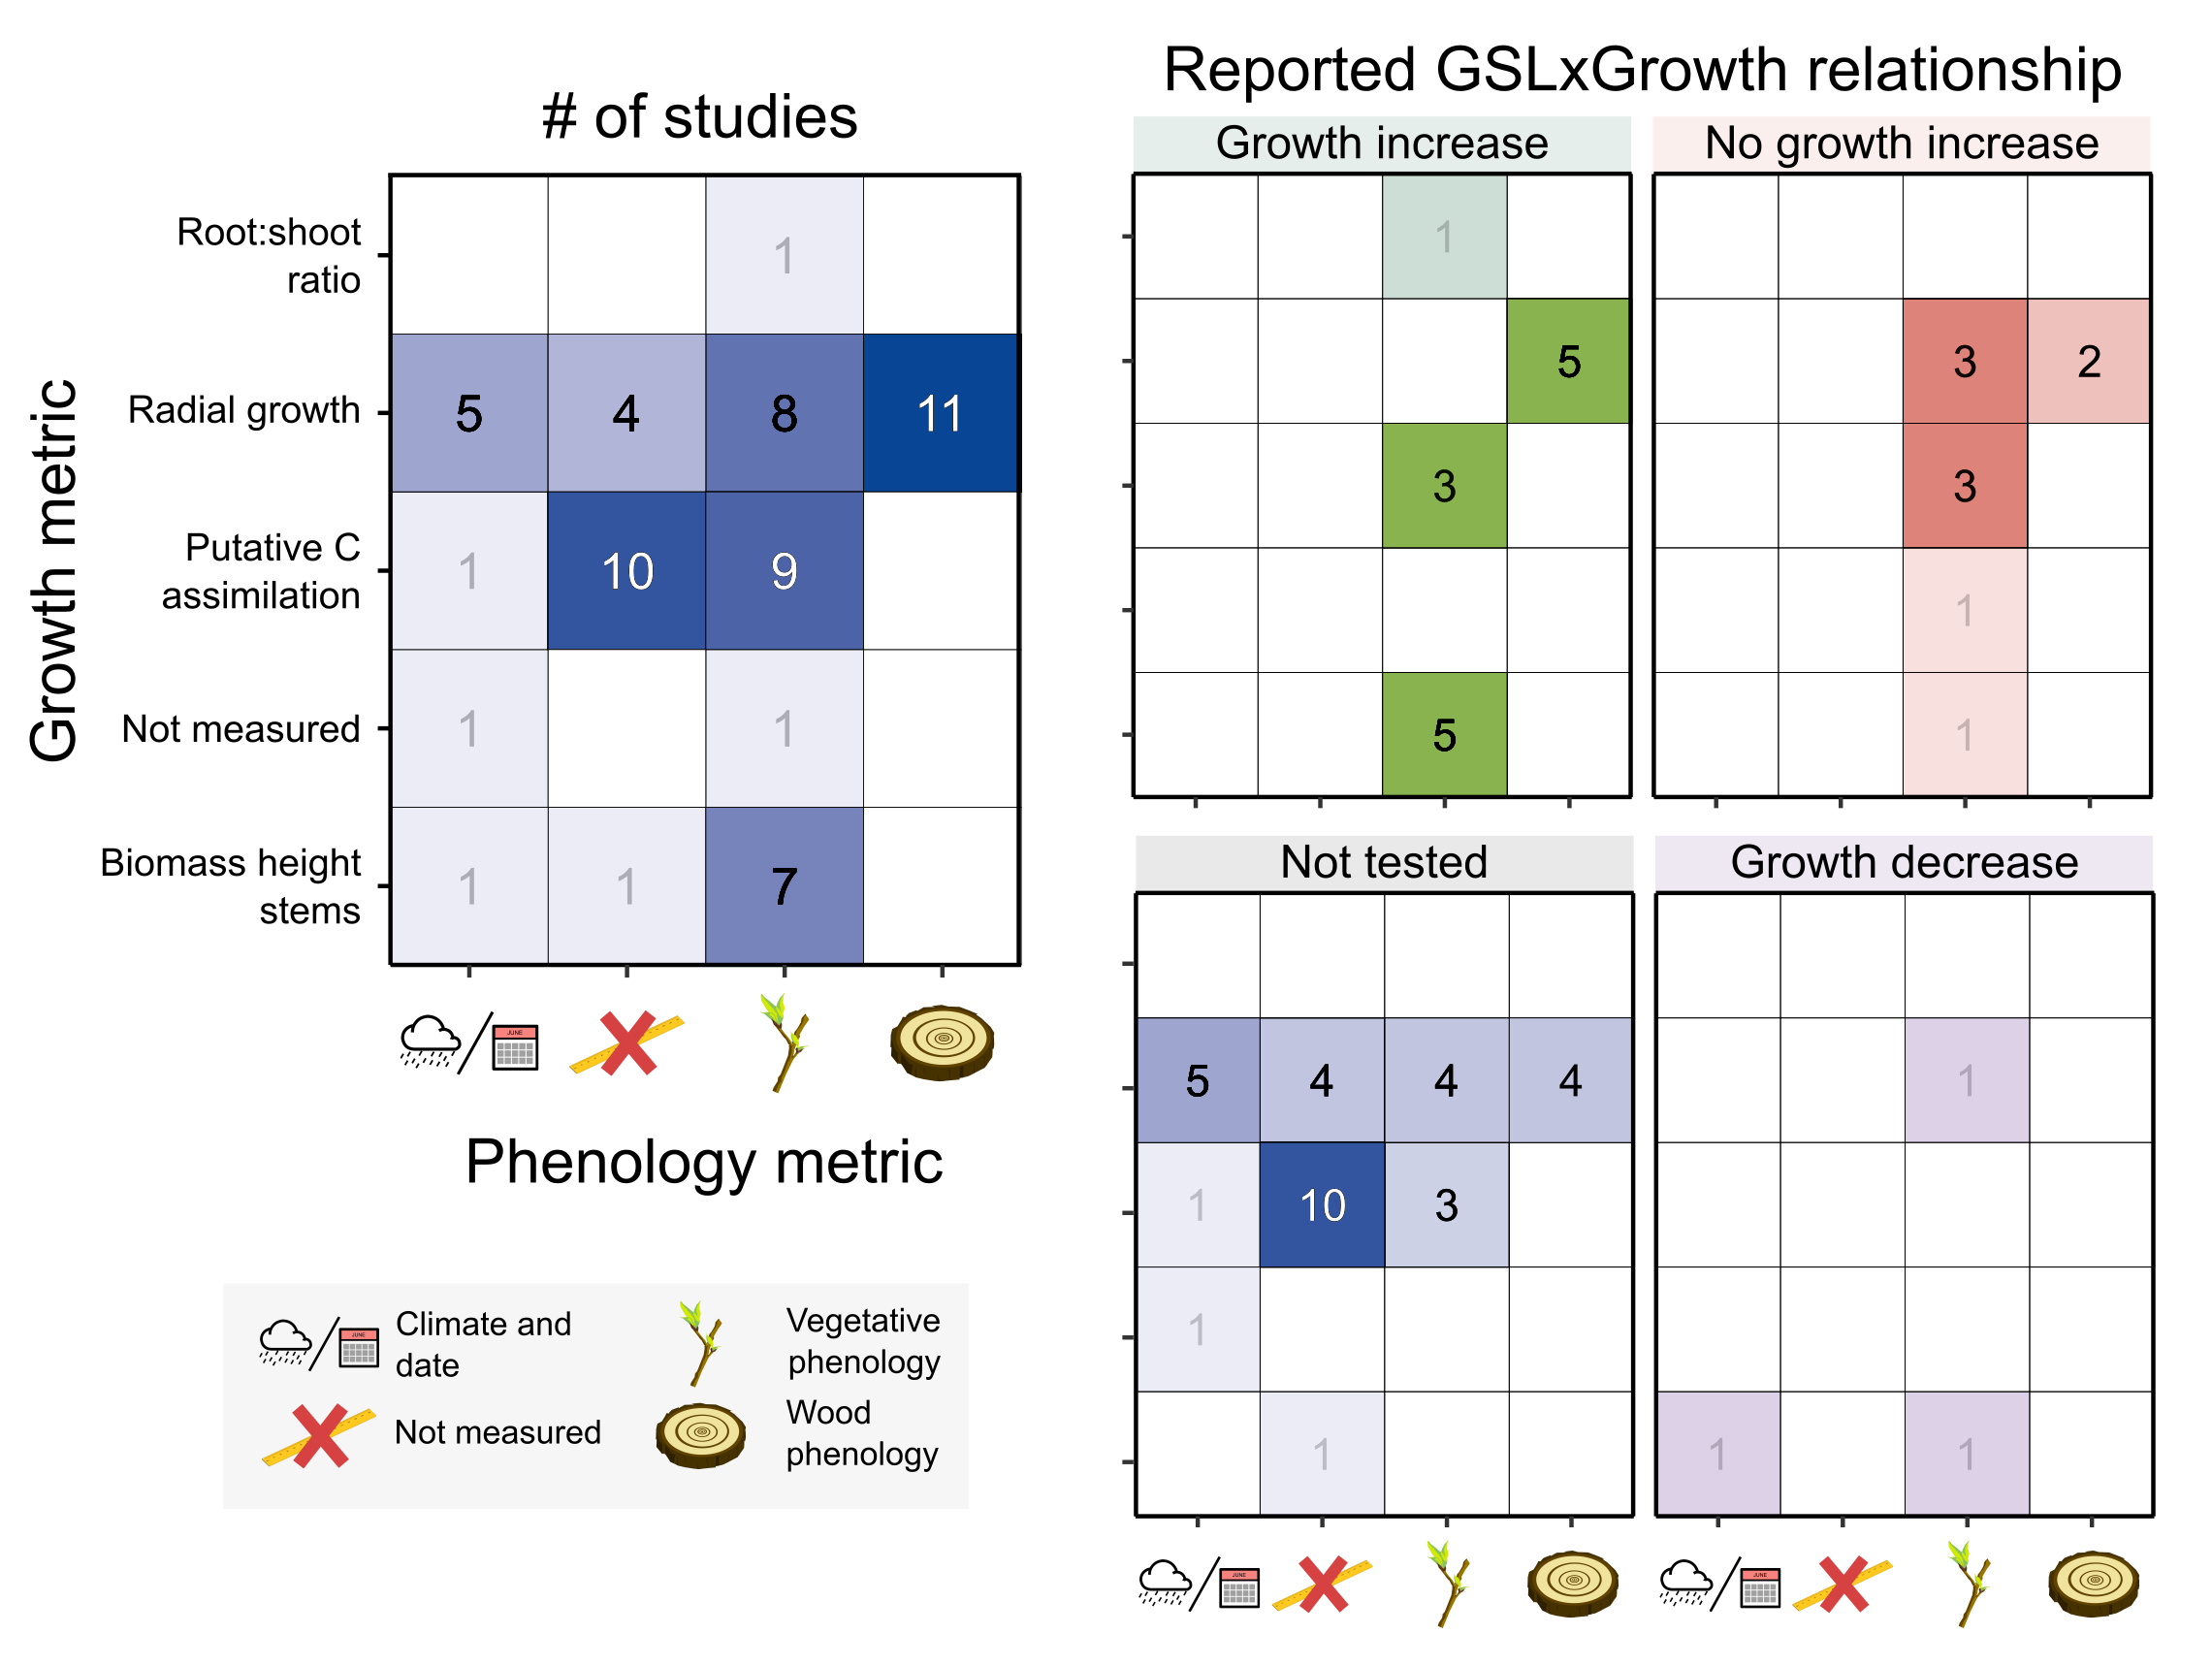
\includegraphics[width=1\textwidth]{..//figures/_figuresFromRuben/heatmap.png} % {..//figures/heatmaps/combinedheatmap_gslxgrowth_simple.pdf}
\caption{\emph{Growth $\times$ growing season length relationships across studies and methods.} We found no coherency in which methods did or did not find a positive relationship. A number of studies tested relationships possibly related to growth $\times$ growing season length (e.g. they tested how spring temperatures related to growth) but never directly growth $\times$ growing season length, thus `not tested' was surprisingly common across methods. Left, frequency of phenological metrics and growth metrics used across the reviewed studies. Right, distribution of observed responses across these approaches. The number of papers within each combination is displayed, with shade emphasizing this value. See Supplement for review details.}
\end{figure}

\iffalse
\begin{figure}[h!]
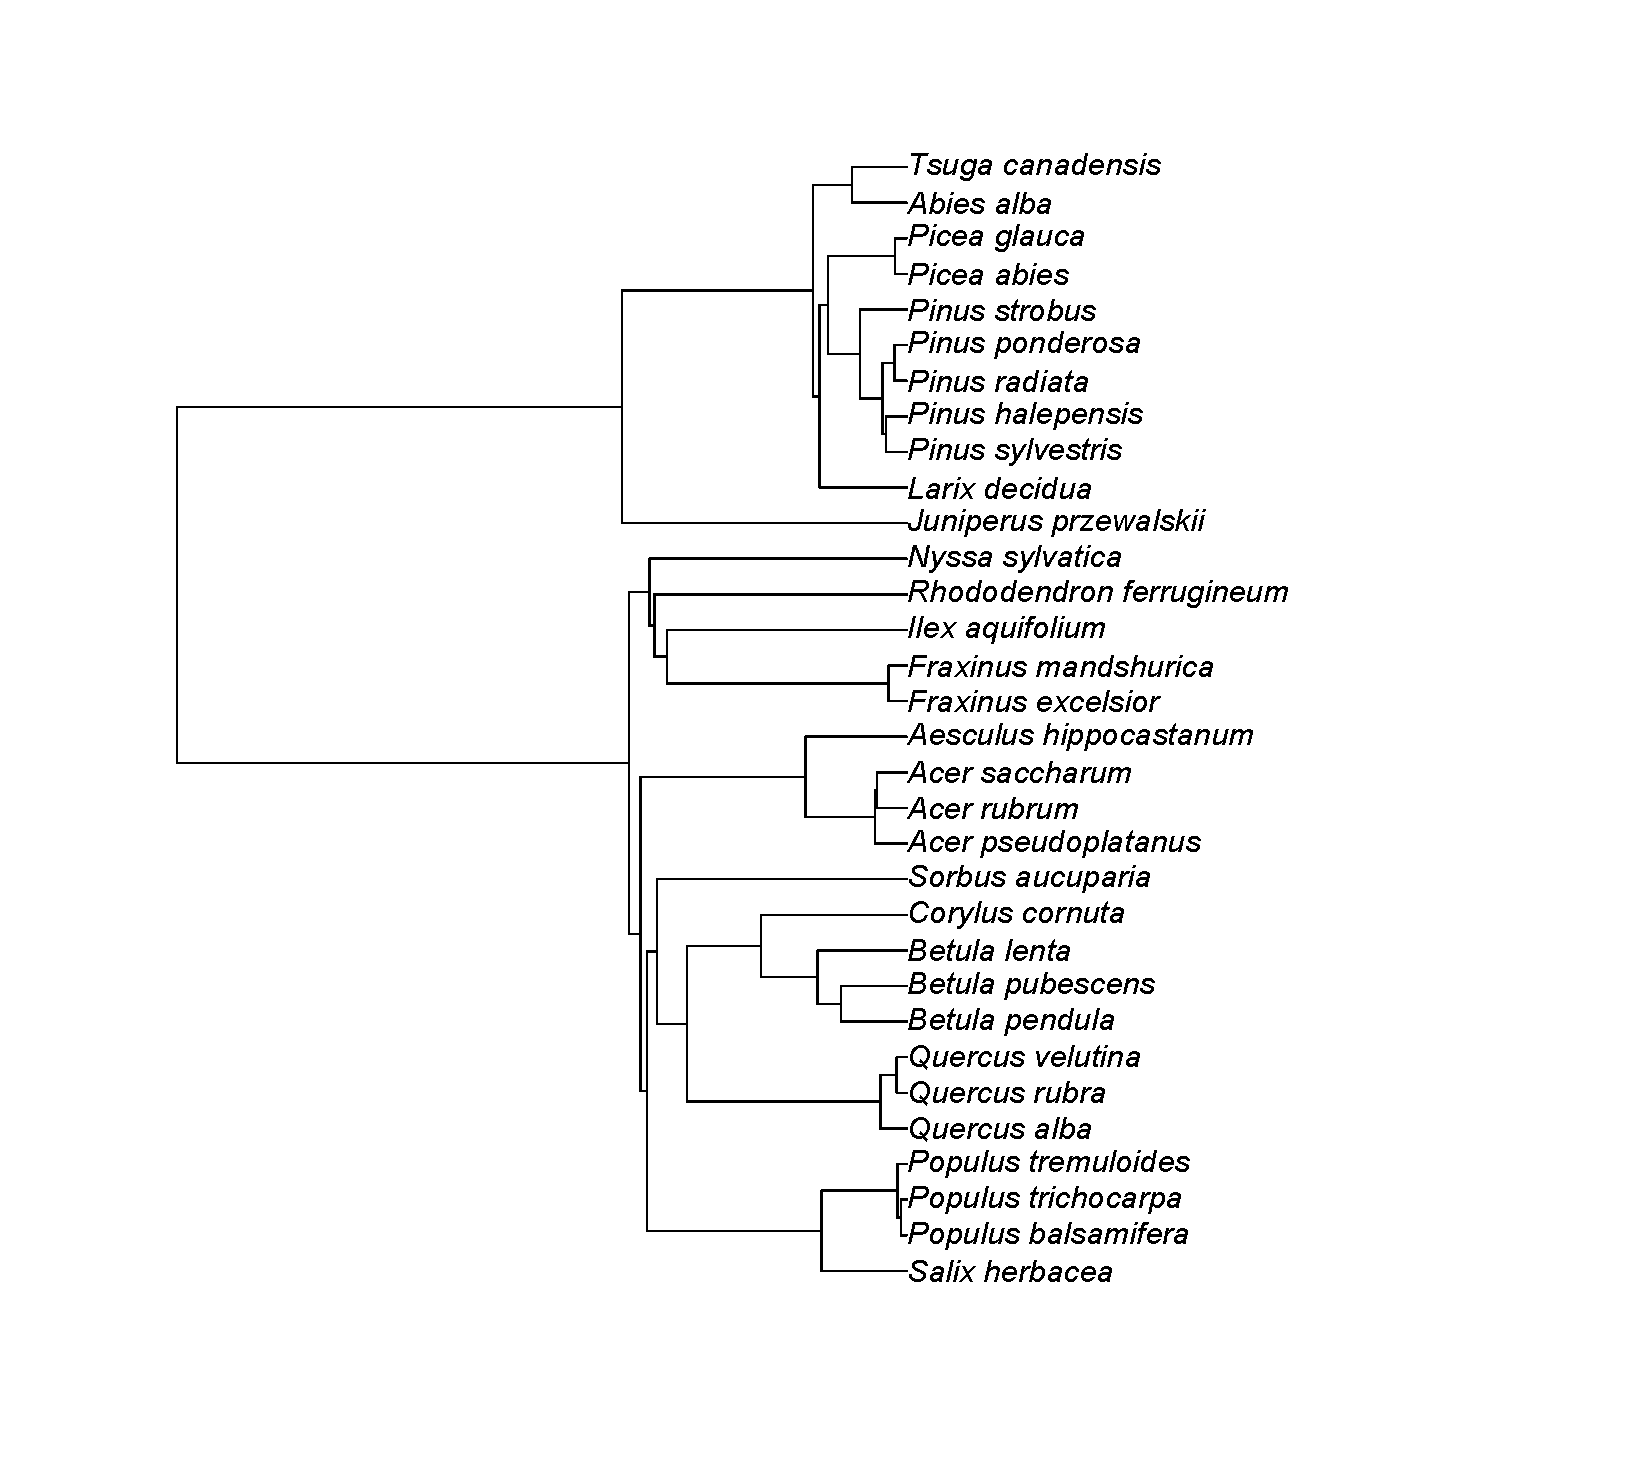
\includegraphics[width=1\textwidth]{..//figures/phylo.pdf}
\caption{We could switch Fig. \ref{fig:sppfinds} from Supp to main text and plot on phylogeny ... I just had time to plot the phylogeny quickly so did not layer on yes/no or find the missing species, like Fagus.}
\label{fig:sppphylo}
\end{figure}
\fi 

\clearpage
\begin{figure}[h!]
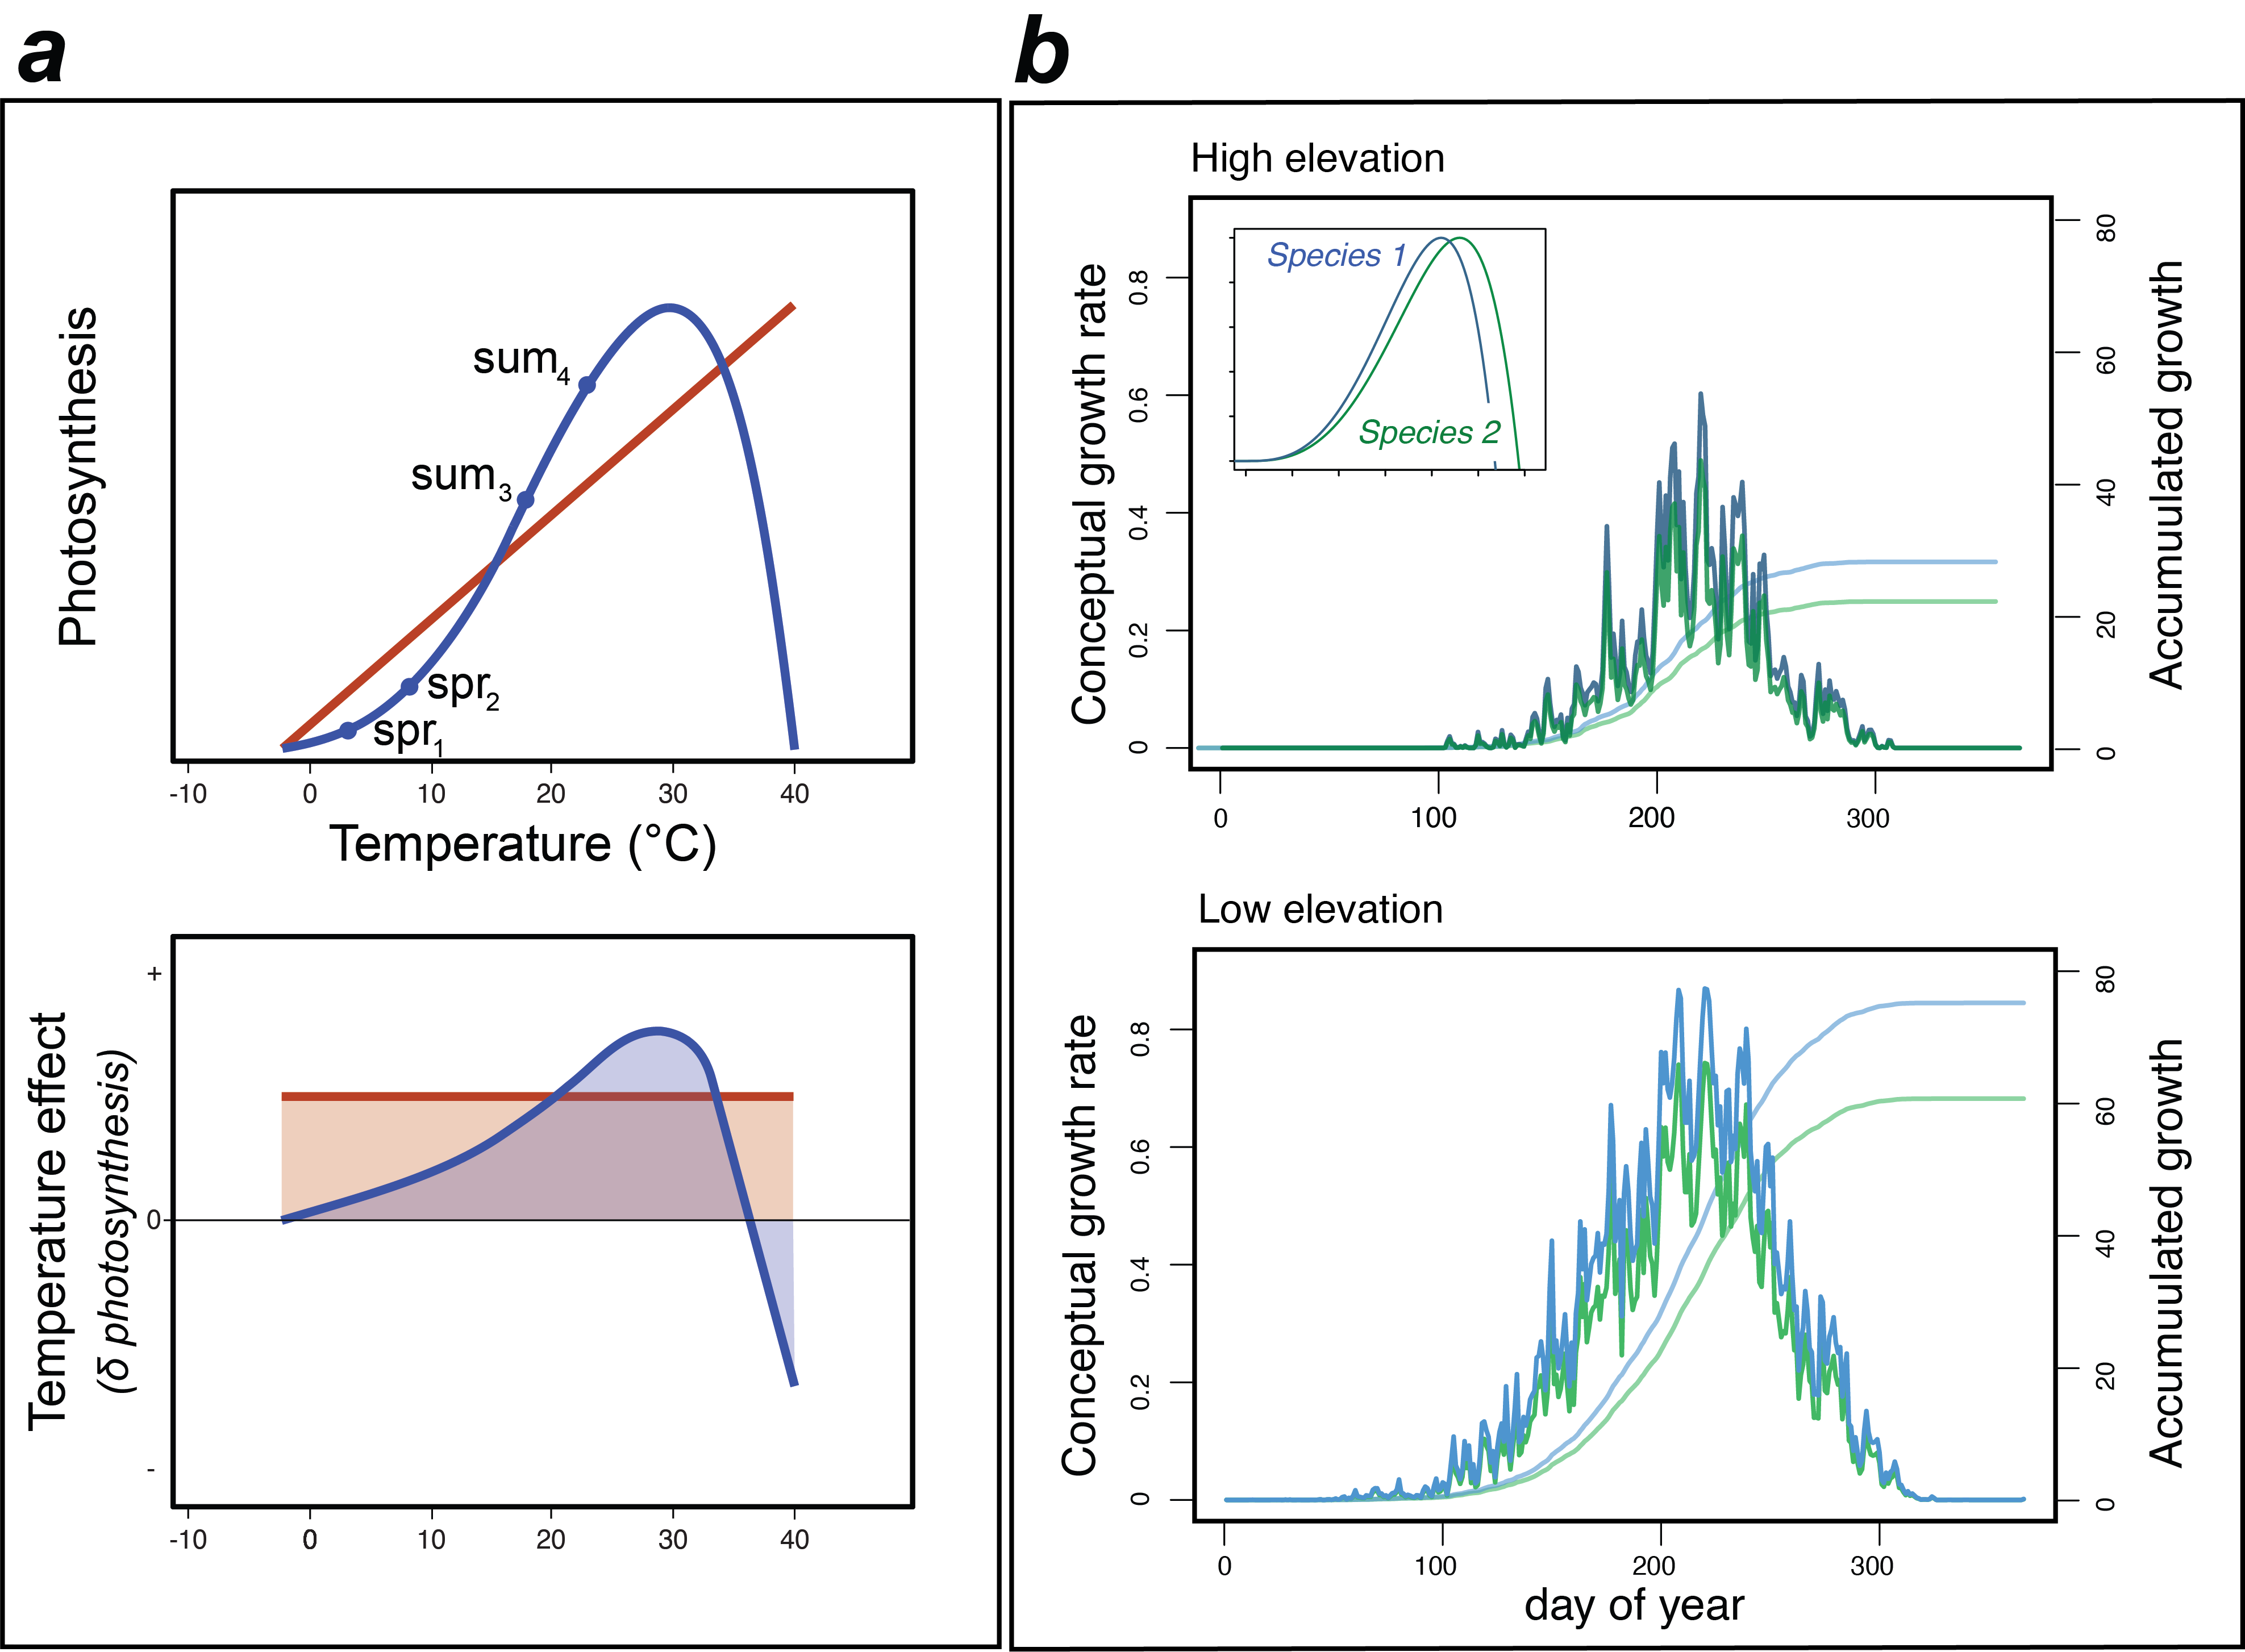
\includegraphics[width=1\textwidth]{..//figures/elevationconcept/elevationrateswtempresponse.png}
\caption{\emph{Understanding how longer seasons with climate change affect growth requires teasing out effects of longer seasons versus warmer seasons.} These two effects generally co-vary in observational data, adding complexity that we show here with two examples. a) A general net photosynthesis response curve (top panel), which has a non-linear response to temperature  \citep[blue curve, adapted from meta-analysis of][]{rezende2019thermal}, contrasts with the commonly used linear response (red). This non-linearity means that increases in lower temperatures---such as those in the spring when much of growing season extensions may happen---have lower absolute increases in photosynthesis compared to increases in later-season (e.g. summer) warmer temperatures, while a linear response assumes a constant scale of effect across low to high temperatures (bottom). b) Conceptual growth responses to temperature for two different species with different growth rate responses to temperature (top, inset), which impacts their growth across the season, leading to small absolute differences in accumulated growth at a conceptual high elevation site (top) versus larger differences in accumulated growth low elevation site (bottom). Testing how growth varies across larger spatial gradients of growing season length, as we conceptualize here (b) could help establish a baseline expectation of the scale of temporal---especially inter-annual variation---and force a greater reckoning with drivers that shift alongside growing season length.}
% \caption{(DRAFT of potential new figure): Testing how growth varies across larger spatial gradients of growing season length could help establish a baseline expectation of the scale of temporal---especially inter-annual variation---and force a greater reckoning with drivers that shift alongside growing season length. This conceptual figure uses data from a cool-weather, temperate site at two elevations (Mount Rainier/Tahoma in USA) with show potential differences in growing season length (dots on top) and biological rates. Other gradients in warmer locations would show much higher rates, but also likely more days where rates are zero due to too high temperatures. Here we estimated growing season length as days above 5\degree C and used an idealized curve (inset) to calculate daily rates. Left shows based on climatic data from the 1980s, while the right is based on 2014-2023. [I could edit this to show TWO species that respond slightly differently to temperature, but then we need to drop one elevation or one time period. THOUGHTS?] }
\label{fig:moraconcept}
\end{figure}

\clearpage
\begin{figure}[h!]
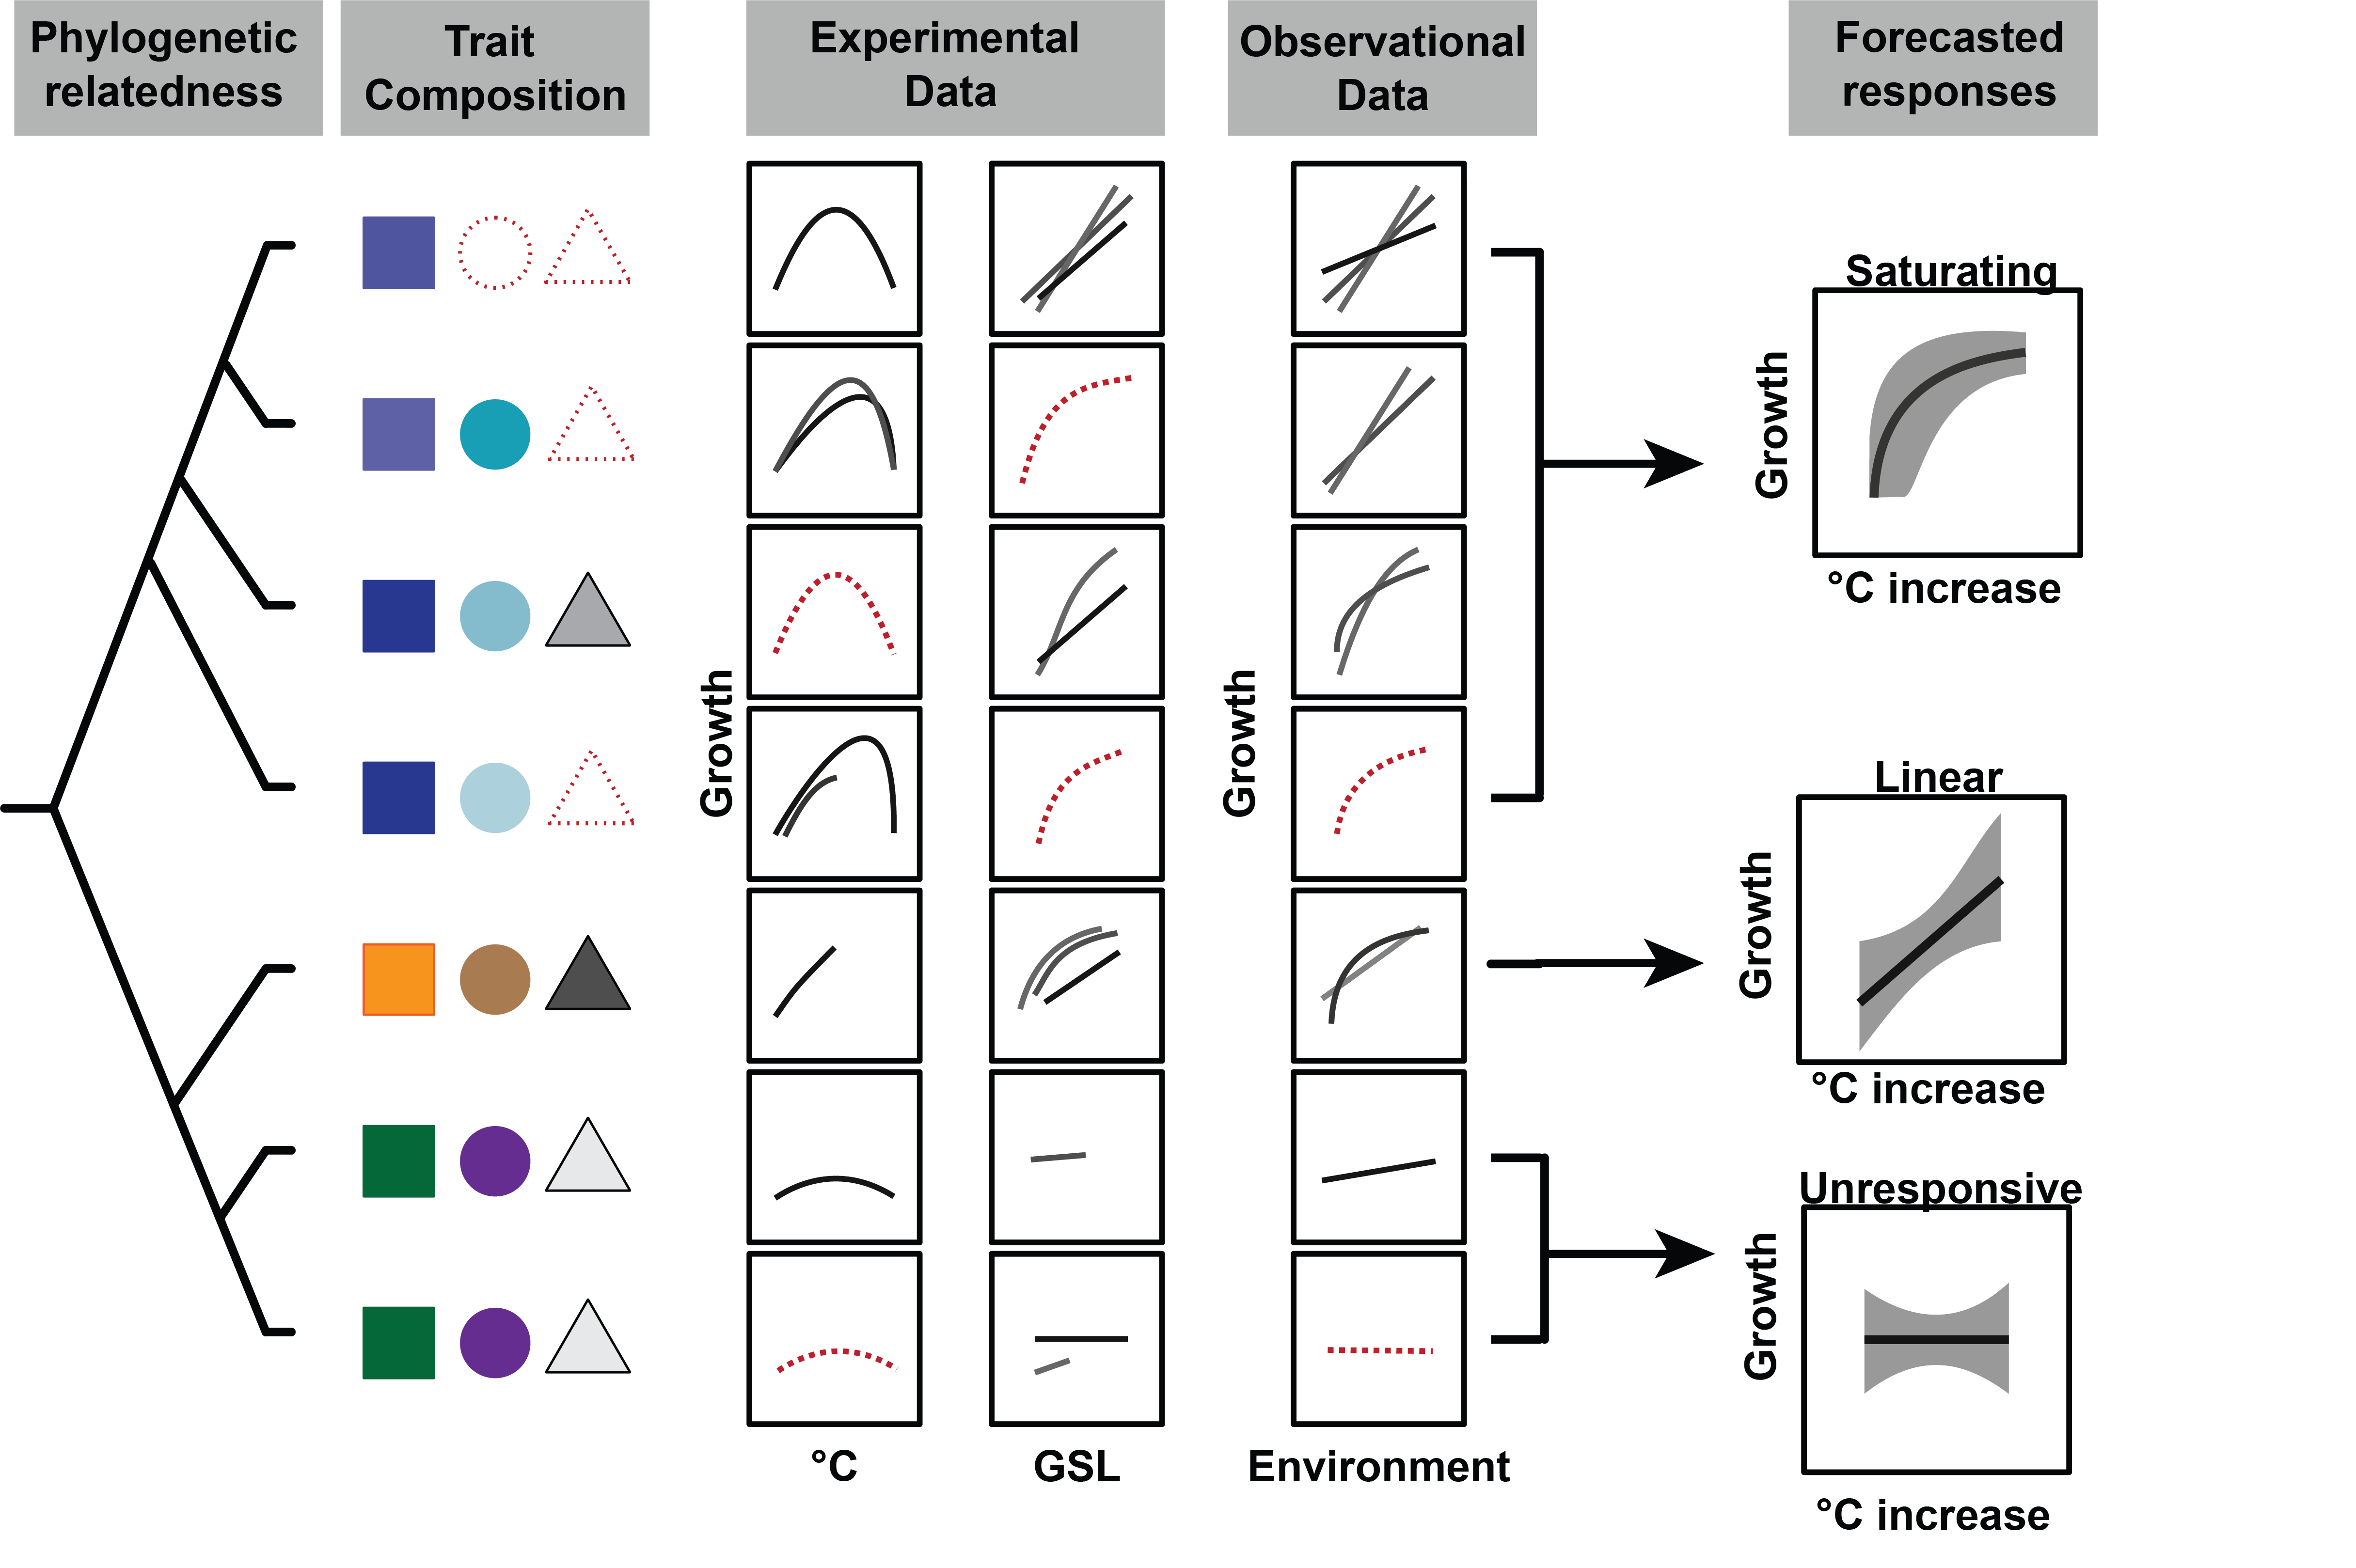
\includegraphics[width=1\textwidth]{..//figures/phylomodel/phylomodel.png}
\caption{\emph{A trait-based phylogenetic model can naturally organize species responses to predict how they respond to longer seasons.} This approach estimates a universal model that is then shaped by species evolutionary history (shown at left via a phylogenetic tree) and traits to produce the divergent responses observed across species (and, not shown, populations) today. We argue this framework can organize and guide experiments that separate out changes in temperature from changes in growing season length (\degree C and GSL in see middle panels) to better integrate observational data and identify different responses by species that can help forecast (see `Building a new framework for growth $\times$ season length' section for more details). It also can be useful for global forecasts. For example, species-level estimates combined with data on species abundance across forests \citep[e.g.][]{FIA,fischer2019swiss} could predict larger-scale metrics, such as satellite observations of phenology and productivity. Here, we show how this approach can identify one clade (top) with a common response to longer seasons that also shares a suite of similar traits, and can identify a unique response by one species in a clade where that species also has a unique trait compared to other species with the same common ancestor (lower clade), while handling uneven sampling and missing data (the dashed red lines represent that the model will predict a response for each species). }  % Similarly traits that co-vary with different responses can be more quickly identified by identifying the common ancestor to species with similar responses!
% Caption could add that traits might include sensitivity to day length, chilling requirements, forcing temperature, deciduous nature, or bud formation. Observational data includes both phenology networks and remote sensing products. 
\label{fig:phylomodel}
\end{figure}


\end{document}
